\chapter{Interférences}
Les interférences sont des phénomènes apparaissant aux points de l'espace où se propagent des ondes générées par des sources différentes. Puisque les effets \footnote{champs électromagnétiques, déplacements,...} en provenance de ces sources s'additionnent vectoriellement en tout point, des effets d'interférence constructive ou destructive sont possibles. L'intensité résultante n'est donc a priori pas égale à la somme des intensités de chaque onde. 

Ces effets sont très importants dans la caractérisation des phénomènes ondulatoires. Dans l'histoire des sciences, ils ont entre autres permis de prouver qu'un phénomène est bien ondulatoire. La preuve que la lumière ne possède pas uniquement un aspect corpusculaire\footnote{théorie initiale élaborée entre autres par Newton} a été apportée par ce principe (voir \textit{expérience de Young}).\\

Dans la grande majorité des cas, lorsque l'on est en présence de plusieurs ondes de sources différentes, le principe de superposition s'applique simplement en additionnant (vectoriellement) les grandeurs des deux ondes. L'ensemble des relations établies dans ce chapitre se basent sur ce principe. Pour être complet, il faut cependant noter que dans certaines situations, des conditions aux limites doivent être prises en compte et peuvent compliquer le raisonnement. Par exemple, supposons que 2 personnes secouent une corde verticalement à ses deux extrémités. Il faut décomposer le déplacement de la corde en 2 et appliquer le principe de superposition pour connaître le déplacement total. Pour le sous-problème de l'onde générée par la personne de gauche, la condition limite impose que le déplacement soit nul à l'extrémité droite. Réciproquement, le deuxième sous-problème possède une condition limite imposant un déplacement nul à l'extrémité gauche de la corde. La combinaison de ces conditions avec le principe de superposition permettent donc à la corde de respecter les déplacements imposés à ses deux extrémités.

\section{Interférence entre deux sources de même fréquence}

\begin{marginfigure}[0cm]
	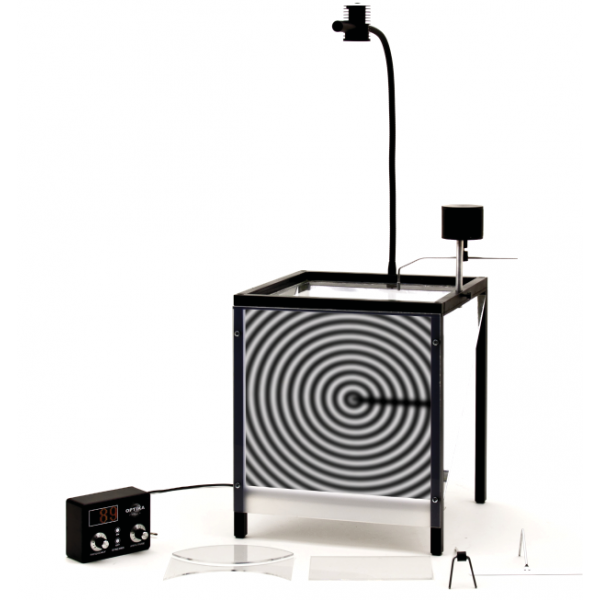
\includegraphics[width=5cm]{cuves-a-ondes}
	\caption{Cuve à ondes}
\end{marginfigure}

L'observation de ce phénomène peut être réalisée sur une cuve à ondes. Celle-ci contient un bac rempli d'eau et surmonté par deux pointes en mouvement vertical sinusoïdal. Deux ondes circulaires sont alors générées par la vibration des pointes qui affleurent l'eau.

Lorsque les pointes oscillent exactement en phase, les deux sources ponctuelles sont dites cohérentes. Pour simplifier les calculs, nous négligeons l'atténuation de leur amplitude avec la distance. Comme indiqué ci-dessus, nous travaillons dans l'hypothèse du principe de superposition, c'est-à-dire que l' onde résultante est la simple somme du déplacement vertical des deux ondes émises par les sources. Ce principe est une bonne approximation, tant que les amplitudes des deux ondes sont faibles. Si les amplitudes deviennent importantes, des non-linéarités apparaissent, mais elles ne seront pas abordées dans ce cours. 

\begin{figure}[htb]
\centering
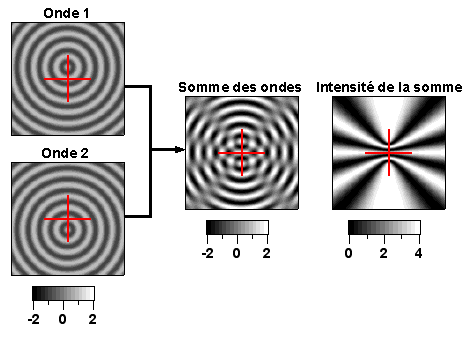
\includegraphics[scale=0.5]{omega}
\caption{Intensité résultante de deux sources ponctuelles}
\label{omega}
\end{figure}

Sur la figure \ref{omega} dont l'animation est disponible sur le site web\footnote{\url{http://perso.uclouvain.be/alain.jonas/Cours/FSAB1203/}}, la somme des deux ondes présente des bandes grises fixes correspondant à une amplitude nulle\footnote{les niveaux de gris sont donnés par les barres sous chaque image}. Dans ces régions, appelées \textit{nodales} où se situent les \textit{noeuds}, l'oscillation est nulle à tous les instants; les deux ondes émises par les sources y interfèrent de manière destructive. Cela se produit quand les maxima des oscillations (les bosses) de la première onde coïncident avec les minima des oscillations (les creux) de la seconde. Entre ces régions, on trouve un comportement ondulatoire typique.

Le graphe de droite représente l'intensité de l'onde résultante qui, pour rappel, représente aussi le flux d'énergie véhiculé localement par l'onde en $W/m^2$, moyenné sur une durée beaucoup plus grande que la période. Contrairement aux trois autres graphes, cette image est fixe, puisqu'il s'agit d'une moyenne sur le temps. Le graphe du milieu lui est semblable car l'intensité est proportionnelle au carré de l'amplitude du déplacement vertical de l'onde, et les bandes d'amplitude nulles correspondent bien aux lignes d'intensités nulles de la figure de droite. Par contre, l'intensité est forte à d'autres endroits, là où les deux ondes primaires interfèrent constructivement: il s'agit des régions \textit{anti-nodales} où se situent les \textit{ventres}, dans lesquelles les maxima de la première onde coïncident avec les maxima de la seconde.\\
 
Analysons tout d'abord le comportement de l'onde résultante sous forme graphique. La figure \ref{point} analyse la valeur de l'amplitude des ondelettes en 3 points à la surface de l'eau.

\begin{figure}[htb]
\centering
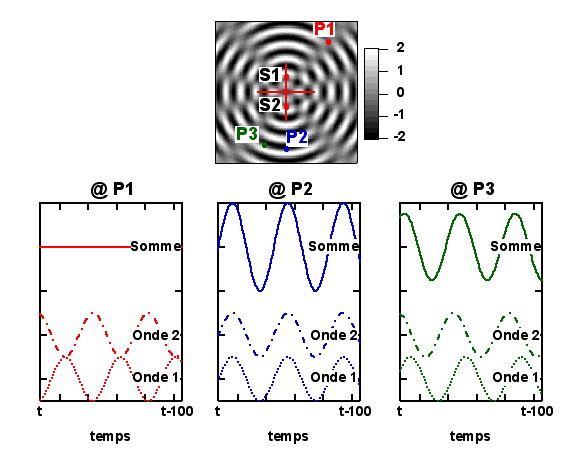
\includegraphics[scale=0.7]{point}
\caption{Analyse des ondulations en différents points à la surface de l'eau}
\label{point}
\end{figure}

L'onde émise en $S_1$ prend moins de temps à atteindre le point rouge ($P_1$) que l'onde émise en $S_2$. Le retard de l'une par rapport à l'autre est tel que les maxima de l'une correspondent aux minima de l'autre, et la résultante est nulle (fig. @P1) : l'interférence est destructive. En $P_2$ par contre, le retard de la première onde par rapport à la seconde est tel que les maxima (et les minima) des deux ondes coïncident. Les ondes interfèrent de manière constructive, et l'amplitude de l'onde résultante est double de celle de chacune des ondes primaires. Enfin, en $P_3$, la situation est intermédiaire.\\

Passons à une description mathématique de ces interférences dans laquelle nous écrivons le champ total en un point $P$ quelconque de l'espace. Les relations ci-dessous conviennent pour le cas simplifié de deux sources ponctuelles cohérentes, de même amplitude, de même longueur d'onde\footnote{dans la cuve à ondes, c'est trivial puisque les ondes se propagent dans le même milieu} et de même polarisation\footnote{dans la cuve à ondes, la polarisation n'a pas de sens puisque la grandeur analysée est scalaire: le déplacement vertical}. Nous considérerons également que les ondes primaires sont des ondes circulaires, polarisées dans la direction de l'axe des $z$ et de forme sinusoïdale.
Le champ créé en $P$ par la première onde est de la forme 
$$A \cos (kr_1-\omega t)\overset\rightarrow{\mbox{l}_z},$$
où $r_1$ est la distance entre la première source et le point $P$, et $k=2\pi/\lambda$ est le nombre d'onde. 

De la même manière, le champ créé en $P$ par la seconde onde est de la forme 
$$A \cos (kr_2-\omega t +\phi_2)\overset\rightarrow{\mbox{l}_z},$$
où $r_2$ est la distance entre la seconde source et le point $P$, et $\phi_2$ est un terme prenant en compte un éventuel déphasage entre les deux sources. 

En $P$, le champ résultant total est donc:

\begin{align*}
\overset\rightarrow{E}(P)&=A \cos (kr_1-\omega t)\overset\rightarrow{\mbox{l}_z} + A \cos (kr_2-\omega t +\phi_2)\:\overset\rightarrow{\mbox{l}_z} \\&
=A \bigg(\cos (kr_1-\omega t)+ \cos (kr_2-\omega t +\phi_2)\bigg)\:\overset\rightarrow{\mbox{l}_z}\\&
=A \bigg(2\cos \Big(\frac{\phi_2 +kr_2-kr_1}{2}\Big)\cos \Big(\frac{\phi_2 +kr_2+kr_1}{2}-\omega t\Big)\bigg)\:\overset\rightarrow{\mbox{l}_z}\\&
=\underbrace{2A\cos \Big(\frac{\phi}{2}\Big)}_\textrm{amplitude}\underbrace{\cos (\phi'-\omega t)}_\textrm{oscillation}\:\overset\rightarrow{\mbox{l}_z}
\end{align*}

où $\phi=\phi_2 +kr_2-kr_1$ et $\phi'=(\phi_2 +kr_2+kr_1)/2$.

Cette fonction possède une partie liée à l'amplitude qui est modulée spatialement par $\cos (\phi/2)$. Ce terme est indépendant du temps et ne dépend donc que de la position du point $P$. La figure d'interférence\footnote{
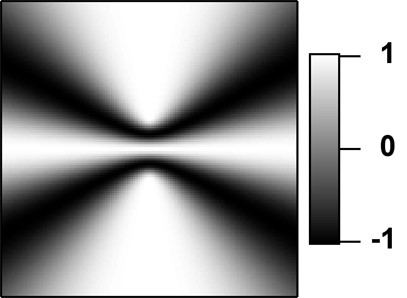
\includegraphics[scale=0.63]{M6}} des deux sources est établie dès la création des premières oscillations.
Le lieu des points de même amplitude est une hyperbole dont les foyers sont les deux sources initiales puisqu'il satisfait
$$2A\cos \Big(\frac{\phi_2 +k(r_2-r_1)}{2}\Big)=Constante.$$
C'est bien l'équation d'une hyperbole, c'est-à-dire l'ensemble des points dont la différence des distantes $r_2-r_1$ est constante.\\

L'onde se déplace suivant des ellipses\footnote{
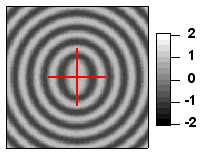
\includegraphics[scale=0.6]{M5}}. En effet, nous cherchons le lieu des points de même déplacement vertical à tout moment, c'est-à-dire les points dont l'argument du cosinus\footnote{partie de $y(P)$ liée au temps} est identique.
En particulier pour $t=0$, le lieu des point devient
$$\phi'=\frac{\phi_2 +kr_2+kr_1}{2}=Constante$$ 
et décrit bien une ellipse, l'ensemble des points dont la somme des distances $r_1+r_2$ est constante.\\

Nous obtenons ensuite une expression pour l'intensité, qui est proportionnelle au carré de l'amplitude:
$$I\propto 4A^2\cos^2 \Big(\frac{\phi}{2}\Big)$$
L'onde résultante en $P$ s'exprime donc comme le produit d'une fonction oscillante qui traduit le caractère ondulatoire de l'onde résultante, et d'une amplitude généralisée. Cette amplitude généralisée fait apparaître $\phi$, qui est le déphasage entre la seconde et la première onde au point P, c'est-à-dire la différence entre la phase de l'onde 2 en P et la phase de l'onde 1 en P. Ces phases résultent de la propagation des ondes sur des distances données (les termes en $kr_i$), et des phases des sources elles-mêmes ($\phi_2$). Le déphasage est une fonction de l'espace, mais pas du temps.

\fbox{\begin{minipage}{1.5\textwidth}
   Lorsque le déphasage vaut un multiple impair de $\pi$,
   \begin{itemize}
   \item $\phi=(2n+1)\pi$ et $\cos(\phi/2)=0$: les ondes interfèrent de manière destructive. C'est le cas en $P_2$.
   \end{itemize}
Si par contre le déphasage vaut un multiple pair de $\pi$, 
\begin{itemize}
   \item $\phi=2n\pi$ et $\cos(\phi/2)=\pm 1$: les ondes interfèrent de manière constructive. C'est le cas en $P_1$.
   \end{itemize}
   
L'intensité
\begin{itemize}
   \item est nulle pour les points auxquels les ondes interfèrent de manière destructive;
   \end{itemize}
          \begin{itemize}
   \item est proportionnelle à $4A^2$ là où les ondes interfèrent de manière constructive
   \end{itemize}

\end{minipage}}\\

L'intensité dans ces régions vaut 4 fois celle de chacune des ondes primaires, soit deux fois plus que la somme des intensités des ondes primaires. L'énergie n'est par pour autant créée, les interférences provoquent une redistribution spatiale de l'énergie: certains endroits sont appauvris (interférences destructives), d'autres sont enrichis (interférences constructives), et l'intégrale sur toute la surface est constante, et vaut la somme des intensités émises par chaque source primaire.

\begin{marginfigure}[6cm]
	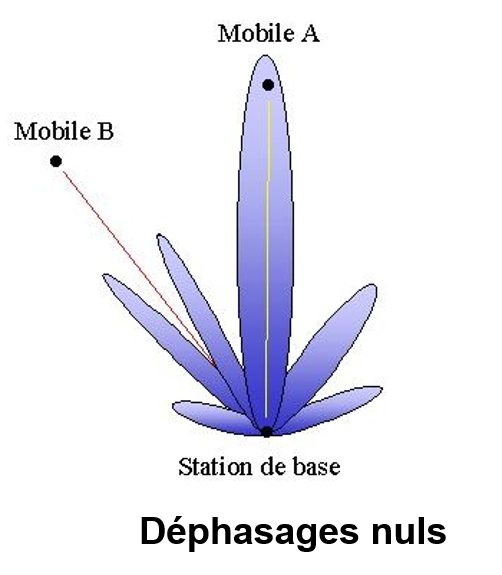
\includegraphics[scale=0.5]{M7}
	\caption{Diagramme polaire}
	\label{fm7}
\end{marginfigure}

Cette redistribution d'énergie permet de diriger l'onde dans une direction préférentielle. Un premier exemple d'application de ce principe sont les casques anti-bruits qui atténuent fortement l'ensemble des bruits extérieurs. Ils possèdent un micro qui analyse le bruit extérieur et qui crée une source qui compense le bruit externe dans la direction du tympan de l'oreille. Une autre application de ce principe se retrouve dans le domaine des télécommunications. En transmission satellite, et plus récemment dans les standards de transmission Wi-fi et 4G, plusieurs antennes sont utilisées conjointement pour choisir des directions préférentielles dans lesquelles on transmet l'information avec une plus grande puissance. Pour ces groupes d'antennes (ou pour les antennes directives telles que les antennes paraboliques), on définit généralement un diagramme de rayonnement (fig \ref{fm7}) qui représente l'intensité qui est envoyée en fonction de la direction. En d'autres termes, la longueur de l'ellipse reflète l'intensité émise ou perçue\footnote{Grâce au principe de réciprocité valable en électromagnétisme, ce diagramme de rayonnement est toujours le même, pour une antenne ou un groupe d'antenne donné, en émission et en réception.} dans cette direction.   Un déphasage\footnote{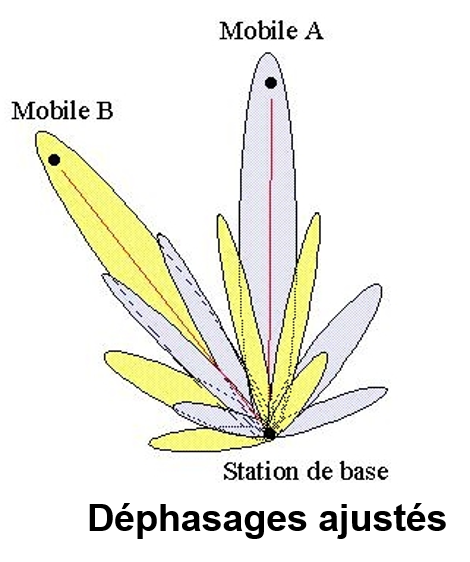
\includegraphics[scale=0.51]{M8}} entre les sources permet alors d'ajuster la direction d'intensité maximale de rayonnement. L'augmentation du nombre d'antennes permet une direction de plus en plus ciblée.
Les systèmes de radioastronomie utilisent aussi depuis longtemps ce procédé pour capter de l'information dans des directions spécifiques en provenance de très longues distances. Des réseaux d'antennes paraboliques sont couramment utilisés.\\

Revenons à notre problème à deux sources. Si les deux sources sont en phase ($\phi_2=0$), le déphasage en $P$ s'écrit $\phi=2\pi(r_2-r_1)/\lambda$, ce qui permet d'écrire les conditions encadrées ci-dessus de la façon suivante:

\fbox{\begin{minipage}{0.9\textwidth}
   Si les deux sources émettent en phase,
   \begin{itemize}
   \item lorsque la différence de chemin $(r2-r1)$ vaut un multiple impair de $\lambda/2$, 
   $$(r2-r1) = (n + 1/2)\lambda,$$ les ondes interfèrent de manière destructive.
             Les maxima de l'une se superposent aux minima de l'autre. 
   \item lorsque la différence de chemin $(r2-r1)$ vaut un multiple pair de $\lambda/2$
   $$(r2-r1) = n\lambda,$$ les ondes interfèrent de manière constructive.
            Les maxima de l'une se superposent aux maxima de l'autre.
   \end{itemize}

\end{minipage}}\\

Dans un grand nombre de cas, on ne s'intéresse pas en détail à l'intensité résultant de l'interférence entre deux sources (ou plus). Ce qui est recherché, c'est le lieu des points où l'intensité est maximale ou minimale, ou encore la longueur d'onde pour laquelle l'intensité est maximale ou minimale à un endroit donné, ou le déphasage à introduire entre deux sources pour avoir une intensité maximale ou minimale en un point donné de l'espace,...

Dans tous ces cas, le problème est réduit et consiste à déterminer les positions et phases des sources, et de calculer la distance entre ces sources et les points considérés. A partir de cela, on détermine le déphasage total, et on applique les règles des encadrés précédents. Examinons deux exemples ci-dessous.\\

Il convient d'énoncer tout d'abord le principe de Huygens sur lequel nous nous appuyons durant les prochains paragraphes:
\begin{center}
\textit{Chaque point atteint par une onde se comporte comme une source secondaire qui émet des ondelettes sphériques dans toutes les directions.}
\end{center}

\begin{figure}[htb]
\centering
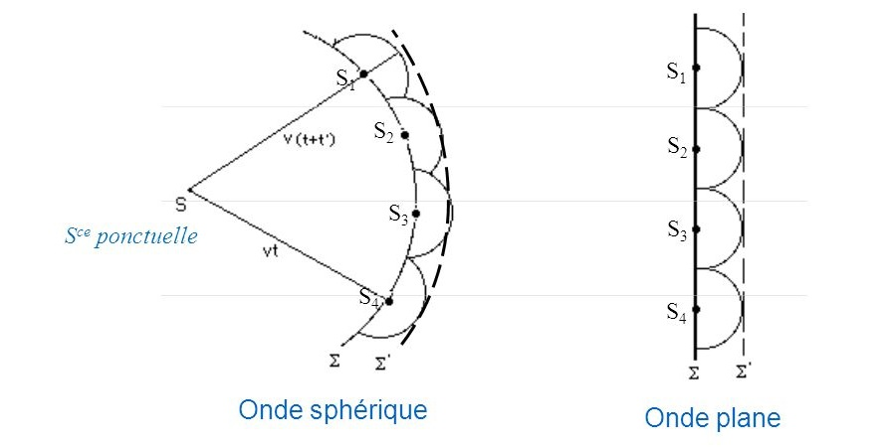
\includegraphics[scale=0.4]{M9.png}
\caption{Principe de Huygens}
\end{figure}

La propagation d'une onde circulaire revient alors à considérer la résultante de toutes les ondelettes circulaires générées à l'instant précédent.
Cet énoncé permet de prédire la position des fronts d’onde un instant plus tard ainsi que de calculer les effets d’interférences et de diffractions de façon suffisamment précise dans des cas simples.
Néanmoins, il est important de mentionner que ce principe est une {\it approximation} pour plusieurs raisons. Premièrement, ce sont en réalité des demi-cercles qui sont formés puisque l'onde résultante ne revient pas en arrière. Et deuxièmement, en pratique, la propagation des ondelettes sphériques ne se fait pas de manière équitable dans toutes les directions. Ce principe a par la suite été ajusté\footnote{au moyen de coefficients ajoutés dans les formules en fonction de la direction de propagation} par Fresnel et Kirchhoff, mais cela sort du cadre de ce cours.\\

Le problème auquel on s'intéresse est celui d'un écran percé de deux fentes infiniment étroites séparées par la distance $d$, illuminé par une onde plane arrivant avec une certaine incidence oblique (fig. \ref{3}). Une vague rencontrant une plaque percée par deux fentes de largeur infinitésimale correspond à ce problème.

\begin{figure}[htb]
\centering
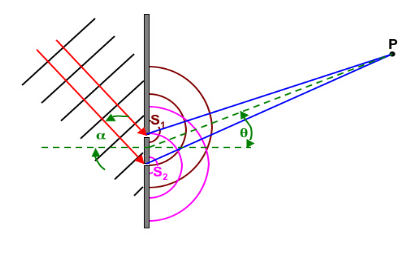
\includegraphics[scale=0.9]{3}
\caption{Interférence entre deux sources cohérentes, crées par l'illumination de deux fentes.}
\label{3}
\end{figure}

Dans ce dessin, les lignes rouges et les lignes bleues n'ont pas d'existence physique réelle. Elles correspondent à des "rayons", qui sont des droites perpendiculaires aux fronts d'onde. Les lignes noires, roses et brunes sont des lignes d'égale phase, par exemple des lignes correspondant aux endroits où le champ est maximal. Ces lignes avancent à la vitesse\footnote{dans le vide; sinon, il faut diviser $c$ par l'indice de réfraction} $c$. Par le principe de Huygens, l'onde plane arrivant vers la plaque se comporte comme deux sources d'ondes se propageant à droite de la plaque. Cette technique est utilisée entre autres pour obtenir deux sources d'ondes exactement à la même fréquence (sources cohérentes) car les ondes sont issues du même front d'onde. Obtenir la même fréquence dans un appareil n'est pas une chose aisée et une différence infime de fréquence peut parfois engendrer des résultats conséquents.\\

Si le point $P$ est situé très loin de l'écran, alors les lignes bleues connectant chacune des fentes au point P sont presque parallèles. 

L'\textit{approximation de Fraunhofer} consiste à considérer que ces droites sont réellement parallèles, une approximation que nous accepterons dans presque tous les exercices de ce cours.

Le déphasage d'une onde à un endroit donné, par rapport à la source, peut s'exprimer facilement en fonction de sa position. Nous le démontrons formellement dans le cas unidimensionnel d'une onde progressive se déplaçant vers la gauche
$$\xi(x,t)=\xi_1\sin(\omega t+kx).$$
En $x=d$, l'onde a pour équation 
$$ \xi(d,t)=\xi_1\sin(\omega t+kd).$$ 
Puisqu'en $x=0$, l'onde vaut 
$$ \xi(0,t)=\xi_1\sin(\omega t),$$ 
l'onde se déphase de $\Delta \phi=kd$ en parcourant une distance $d$. Nous pouvons dès lors en déduire la relation:
$$\Delta\phi=kd\Rightarrow\frac{\Delta\phi}{2\pi}=\frac{d}{\lambda}$$ 


Il est évident qu'il y a deux sources dans le problème, $S_1$ et $S_2$, correspondant aux sources des ondes émises par les fentes lorsqu'elles sont illuminées par l'onde plane. Ces deux sources n'émettent pas en phase, parce que l'onde plane arrive en $S_2$ un peu plus tard qu'en $S_1$. 
Calculons ce retard de phase entre les deux sources.\\

La distance supplémentaire\footnote{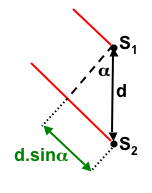
\includegraphics[scale=1]{7}} $d'$ parcourue par l'onde plane pour atteindre $S_2$ vaut $d\sin\alpha$. Compte-tenu du fait qu'une distance d'une longueur d'onde correspond à un déphasage de $2\pi$, le retard de phase de S2 par rapport à S1 est de 
$$ \phi_2=\frac{2\pi}{\lambda}d\sin\alpha.$$ 
Notons que la longueur d'onde dépend du milieu de propagation et ne correspond pas toujours à $c/f$.

Calculons à présent la différence de chemin\footnote{
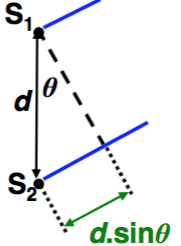
\includegraphics[scale=1]{2}} entre le point $P$ d'observation et les deux sources. Par l'approximation de Fraunhofer, elle ne dépend que de l'angle, et pas des coordonnées détaillées du point $P$: $r_2-r_1=d\sin\theta$.
Le déphasage résultant de cette différence de chemin vaut 
$$k(r_2-r_1)=\frac{2\pi}{\lambda}d\sin\theta.$$ 
Nous retrouvons une expression analogue à la précédente.\\

Il ne reste plus qu'à sommer ces deux termes pour obtenir le déphasage total, en faisant attention à prendre les bons signes pour les déphasages. Ici, $S_2$ est atteint plus tard par l'onde incidente, et le rayon émis par $S_2$ doit parcourir un chemin plus long pour atteindre $P$ que celui émis par $S_1$. Donc, il faut additionner les déphasages à l'incidence et à l'émission. La différence de phase totale est donc 
$$\phi=\frac{2\pi d}{\lambda}(\sin \theta +\sin \alpha).$$
Si cette différence vaut un multiple pair de $\pi$, l'interférence en $P$ est constructive; si elle vaut un multiple impair de $\pi$, l'interférence en $P$ est destructive. A partir de ces conditions, on peut dériver des conditions sur les angles ou la longueur d'onde de telle sorte que l'intensité soit nulle ou maximale à un endroit donné de l'espace. Par exemple, si on cherche les angles pour lesquels il y a interférence constructive avec $\alpha=0$ (incidence normale), on trouve: 
$$ \frac{2\pi d}{\lambda}\sin \theta=2m\pi$$
$$ \Rightarrow d \sin \theta =m\lambda$$
 où $m$ est un nombre entier, positif ou négatif. \\
 
 Si nous plaçons un écran derrière les deux fentes, nous verrons une succession de bandes claires\footnote{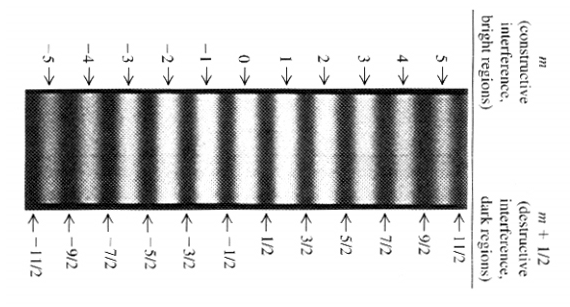
\includegraphics[scale=0.3]{8} Il s'agit ici du cas où les deux fentes sont des minces fentes verticales, les deux sources cohérentes sont dès lors approximativement cylindriques.} appelées franges d'interférence, chaque frange correspondant à une valeur entière de $m$. Cette expérience a été réalisée pour la première fois par Thomas Young\footnote{Médecin anglais, savant polyvalent (archéologue, philologue, physicien des matériaux [le module de Young],…).
 Il lit à 2 ans, et parle 10 langues à 16 ans (dont le Chaldéen, le Syriaque, le Turc et le Perse).} en 1801. Ce scientifique est le premier Anglais à contester la vision corpusculaire de Newton grâce à de multiples expériences sur les phénomènes d'interférences. Il a entre autres expliqué les anneaux de Newton\footnote{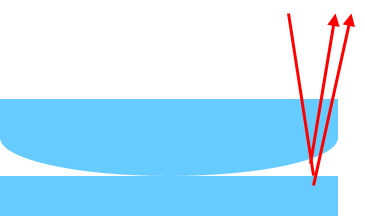
\includegraphics[scale=0.7]{M10} Un anneau de Newton désigne la figure d'interférence obtenue en plaçant une lentille sur une surface plane (voir section suivante).}, ainsi que la couleur des bulles de savon, et le phénomène d'interférence (deux ou plusieurs fentes), à partir d'une théorie ondulatoire. Ses découvertes n'ont pas été acceptée par la plupart des scientifiques car la théorie de Newton semblait décrire parfaitement la physique du monde et ne pouvait donc pas être remise en question.
 

% Les particules adoptent une distribution d’ensemble corrélée mais elles s’ignorent entièrement. En effet, la figure d'interférence\footnote{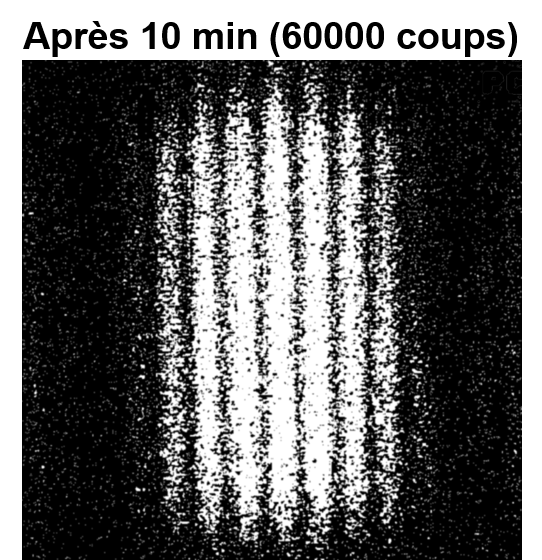
\includegraphics[scale=0.3]{M11} \\Évènements discrets: arrivée de photons (particules) selon une distribution de probabilité donnée par l'intensité du champ (onde).} issue d'une faisceau de particules apparaît aussi lorsque les particules sont envoyées l'une après l'autre. Dans ces conditions, il faut soit que les photons se comportent comme une onde, ou alors qu’ils obéissent de manière aléatoire à une loi statistique décrite par les formules d’interférence.


\section{Film illuminé par une onde plane}
\label{film_onde_plane}

Le second problème est le suivant: un film mince déposé sur un support plan est illuminé par une onde plane sinusoïdale. Cette onde plane rencontre plusieurs interfaces\footnote{par exemple les surfaces d'un polymère multicouche}, en se réfractant et se réfléchissant partiellement à chaque interface. Chaque faisceau réfracté et réfléchi peut lui-même rencontrer plusieurs interfaces, et se réfléchir ou se réfracter partiellement. On aboutit à une multitude d'ondes superposées, et donc à des interférences, comme illustré schématiquement sur la figure \ref{fig:film_mince}.

\begin{figure}[htb]
\centering
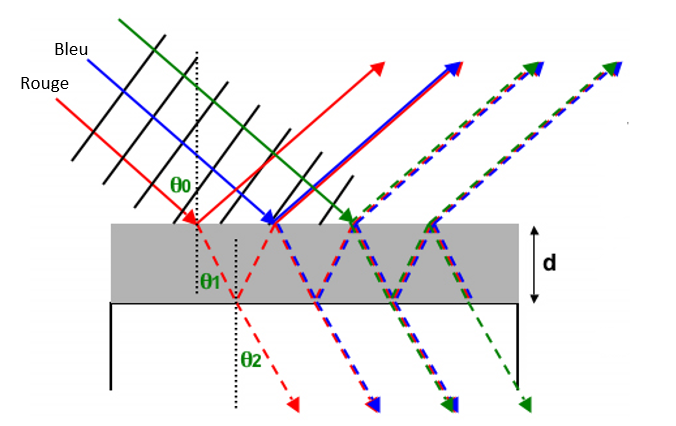
\includegraphics[scale=0.6]{9}
\caption{Interférences issues d'un film mince}
\label{fig:film_mince}
\end{figure}

Les longueurs d'ondes associées à chaque milieu sont données par:
\begin{itemize}
    \item Milieu supérieur $0$ ($n=n_0$): $\lambda_0=\lambda/n_0$
    \item Milieu moyen $1$ ($n=n_1$): $\lambda_1=\lambda/n_1$
    \item Milieu inférieur $2$ ($n=n_2$): $\lambda_2=\lambda/n_2$
\end{itemize}
où $\lambda$ correspond à la longueur d'onde dans le vide.

La loi de Snell permet d'écrire la relation
$$ n_0\sin \theta_0=n_1\sin \theta_1=n_2\sin \theta_2.$$

Dans la figure \ref{fig:film_mince}, trois rayons particuliers appartenant à l'onde sont tracés \sidenote[][-2cm]{il en existe une infinité, mais la situation se reproduit avec la même géométrie pour chacun des autres rayons pris deux à deux}. Les lignes noires sont les lignes de crête \sidenote[][0cm]{elles ne sont pas représentées pour les ondes réfléchies et réfractées, pour ne pas encombrer le dessin}. Concentrons-nous sur deux rayons, le rouge et le bleu, et à leurs deux réflexions qui interfèrent en émergeant du film. 

Pour atteindre le film, le rayon bleu parcourt une distance $a$ supplémentaire par rapport au rayon rouge. Par contre, le faisceau rouge (qui est réfracté, réfléchi puis de nouveau réfracté) atteindra le même point d'émergence que le premier faisceau réfléchi bleu, après avoir effectué un zig-zag\footnote{
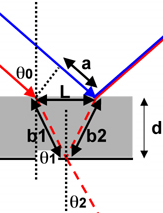
\includegraphics[scale=1]{4}} supplémentaire dans le film, de longueur totale $b=b_1+b_2 = 2b_1$. 

La situation se présente donc comme suit:
\begin{itemize}
    \item Retard de phase dû au chemin $a$:
    $$ \frac{2\pi}{\lambda_0}a=\frac{2\pi}{\lambda_0}L\sin \theta_0=\frac{2\pi}{\lambda_0}2d \tan \theta_1 \sin \theta_0$$
    \item Retard de phase dû au chemin $b$:
    $$\frac{2\pi}{\lambda_1}b=\frac{2\pi}{\lambda_1}\frac{2d}{\cos \theta_1}=\frac{2\pi n_1}{n_0\lambda_0}\frac{2d}{\cos \theta_1}$$
\end{itemize}
Le retard du faisceau rouge par rapport au faisceau bleu est donc:
\begin{align*}
\phi_1 & = \frac{4\pi n_1}{n_0\lambda_0}\frac{d}{\cos \theta_1}-\frac{4\pi}{\lambda_0}d \tan \theta_1 \sin \theta_0 \\
& = \frac{4\pi d}{\lambda_0 \cos \theta_1}\Big (\frac{n_1}{n_0}-\sin \theta_1 \sin \theta_0\Big ) \\
& = \frac{4\pi d}{n_0\lambda_0 \cos \theta_1}\big (n_1-\sin \theta_1 n_0\sin \theta_0\big )\\
& = \frac{4\pi d}{n_0\lambda_0 \cos \theta_1}\big (n_1- n_1\sin^2 \theta_1\big )\\
& = \frac{4\pi dn_1}{n_0\lambda_0 \cos \theta_1}\big (1- \sin^2 \theta_1\big )\\
& = \frac{4\pi dn_1}{n_0\lambda_0 }\cos \theta_1
\end{align*}

En plus de $\phi_1$, il faut rajouter un éventuel déphasage que subirait les ondes en se réfléchissant ou en passant à travers les interfaces. En ce qui concerne leur passage à travers les interfaces, les coefficients de transmission de Fresnel sont toujours positifs \footnote{pour des corps isolants}, et il n'y a pas de déphasage supplémentaire à prendre en compte lors de la traversée d'une interface. Par contre, les coefficients de réflexion de Fresnel peuvent être positifs ou négatifs, selon l'angle d'incidence, la polarisation et la valeur des indices de réfraction des matériaux de part et d'autre de l'interface. S'ils sont négatifs, cela correspond à un déphasage supplémentaire de $\pi$ lors de la réflexion. S'ils sont positifs, il n'y a pas de déphasage supplémentaire. Il faut donc examiner les signes des coefficients de réflexion de Fresnel pour l'interface $0/1$ où se réfléchit le faisceau bleu, et pour l'interface $1/2$ où se réfléchit le faisceau rouge lors de son zig-zag dans le film. Le déphasage total dû aux réflexions vaudra $0$ ou $\pi$.\\

En fin de compte, le déphasage total s'écrit:
$$\phi=\frac{4\pi dn_1}{n_0\lambda_0 }\cos \theta_1+(0\mbox{ ou }\pi).$$
Les conditions d'interférence constructive/destructive correspondent aux cas pour lesquels cette différence de phase est un multiple pair/impair de $\pi$. En connaissant l'angle d'incidence, il est donc possible de calculer les longueurs d'onde éteintes par interférence destructive, ou celles qui sont renforcées par interférence constructive, et expliquer les couleurs du film en fonction de l'angle sous lequel on le regarde. C'est en se basant sur ce principe que l'on peut
fabriquer des couches anti-reflets ou, au contraire, des couches réflectrices.\\

Pour les fréquences dont le déphasage $\phi$ vaut un multiple de $2\pi$, l'onde interfère constructivement et la couleur liée à cette fréquence est mieux perçue. A l'opposé, les ondes qui interfèrent de manière destructive ont leur couleur associée qui est peu visible après la réflexion.

\subsection{Couche anti-reflets}

Des stries sont présentes à la surface de l'oeil de certains insectes pour éviter la réflexion de certaines couleurs à un certain angle d'absorption de la lumière solaire\footnote{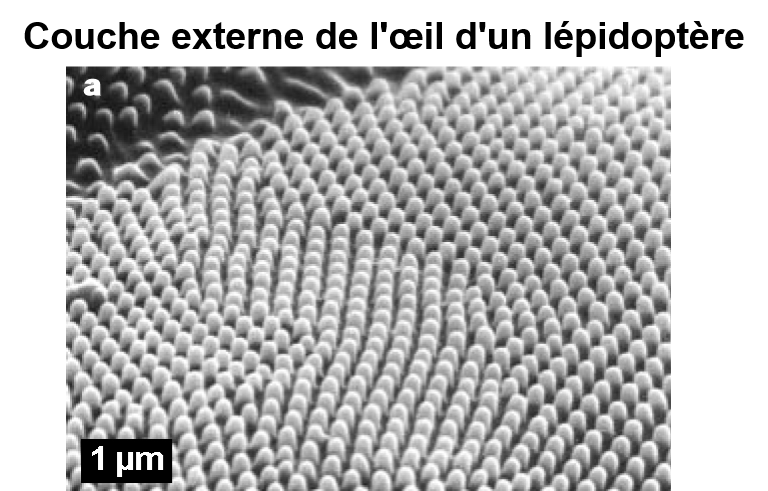
\includegraphics[scale=0.3]{M12}}. L'indice de réflexion de l'oeil d'un lépidoptère valant environ 1.5, les interstices à la surface de l'oeil diminue l'indice de réflexion à environ 1.3 puisqu'il devient plus proche de celui de l'air. Il s'agit donc du problème précédent pour lequel la couche vaut 300 nm. En outre, le gradient de cet indice de réflexion permet spécialement de minimiser la réflexion. Cette couche permet de maximiser la lumière visible rentrant dans l'oeil de l'insecte. Elle présente aussi un réel avantage pour la survie puisqu'elle n'attire pas les prédateurs qui percevraient de la lumière réfléchie. Les couches anti-reflets sur les lunettes\footnote{ou les cellules solaires, \ldot} utilisent ce même principe un peu plus simplifié.
\newpage

\subsection{Couche réflectrice}

Dans le cas contraire, les ailes de certains papillons\footnote{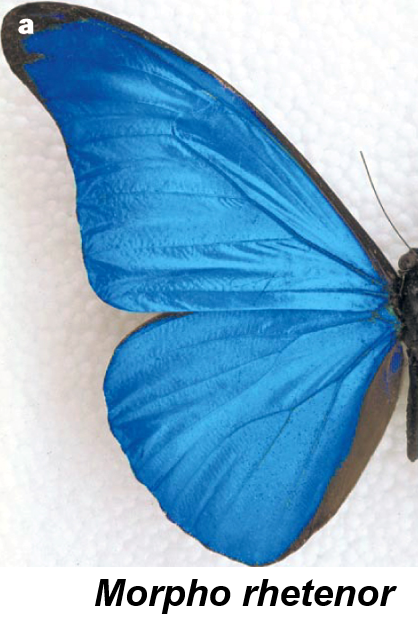
\includegraphics[scale=0.3]{M13}} peuvent être élaborées pour diffuser un maximum de lumière pour certaines couleurs. Les interférences constructives sont maximisées dans le bleu pour que le \textit{Morpho rhetenor} soit vu à 700 m (avantage reproductif).	Par ailleurs, les réflexions désorientent les prédateurs (avantage pour la survie). Les couches réfléchissant la chaleur\footnote{liée à la transmission des rayons infra-rouges} tirent profit ce principe.

\subsection{L'interféromètre de Michelson-Morley}

Michelson était un scientifique de la fin du 19e siècle qui s'est beaucoup intéressé au calcul de la vitesse de la lumière. A cette époque, les gens pensaient que celle-ci se déplaçaient dans un certain milieu\footnote{Personne n'avait encore réussi à le détecter} appelé l'éther. Michelson a donc essayé de calculer la vitesse de la lumière dans cet éther pour prouver son existence. Son raisonnement est établi par analogie avec la vitesse du son qui diffère suivant la direction du vent. Le temps pour faire un aller-retour est légèrement plus court pour la direction perpendiculaire au vent que la direction parallèle. 

\begin{figure}[htb]
\centering
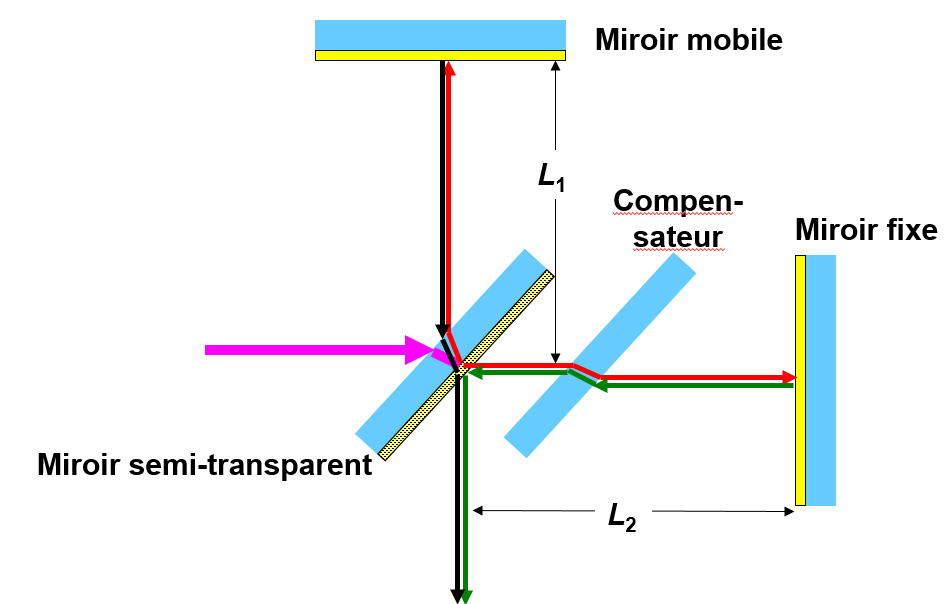
\includegraphics[scale=0.3]{M14}
\caption{Interféromètre de Michelson}
\label{fig:Michelson}
\end{figure}

Puisque la Terre tourne autour d'un axe fixe, la lumière devrait avoir deux vitesses différentes suivant que son trajet se déroule parallèlement ou perpendiculairement à l'axe rotation de la Terre.  Il a donc mesuré les temps mis par chaque trajet en analysant les signaux d'interférences additionnés et projetés sur le miroir fixe.\\

Michelson n'a jamais pu mettre en évidence une différence entre les deux trajets. Ce résultat négatif a amené Lorentz et Einstein à postuler l'inexistence de l'éther et l'invariance de la vitesse de la lumière.






\section{Intensité de la figure d'interférence}

Dans certains cas, il faut non seulement identifier les conditions d'interférence constructive ou destructive, mais aussi calculer l'intensité de l'onde résultante à différents points de l'espace. Ceci est plus difficile que ce que nous avons fait jusqu'ici, puisqu'il faut additionner les champs, puis calculer l'intensité de l'onde résultante\footnote{pour rappel, l'intensité d'une onde est le flux moyen d'énergie passant par unité de surface dans la direction de propagation de l'onde}.\\
 % On peut aussi le calculer en évaluant la norme du vecteur de Poynting $E\times H$ moyenné sur une durée beaucoup plus grande que la période.

Pour simplifier le calcul, il est utile de passer à une représentation différente des ondes sinusoïdales, une représentation sous forme complexe. Considérons une onde électromagnétique de la forme\footnote{il est toujours possible de l'écrire localement sous cette forme, en choisissant correctement son repère; si l'onde est sphérique, $A$ est une fonction de la distance à la source, $x$, mesurée le long d'un rayon; si l'onde est plane, $A$ est une constante} $\overset\rightarrow{\mbox{E}}(x,y,z)=A\cos(kx-\omega t)\overset\rightarrow{\mbox{l}_z}$. Il est évident que nous pouvons aussi écrire:
$$\overset\rightarrow{E}(x,y,z)=\operatorname{Re}\Big((A\exp\big(j(kx-\omega t)\big)\overset\rightarrow{\mbox{l}_z}\Big)=\operatorname{Re}\Big(\overset\rightarrow{E_c}(x,y,z)\Big)$$
où $\operatorname{Re}(c)$ désigne la partie réelle d'un nombre complexe et $j$ est la racine carrée de $-1$. Écrire l'onde $\overset\rightarrow{E}$ sous cette forme revient en fait à la considérer comme la projection sur l'axe réel d'un champ complexe $\overset\rightarrow{E}_c$ tournant dans un plan imaginaire\footnote{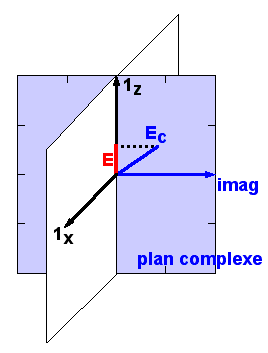
\includegraphics[scale=0.4]{10}} sans existence physique. Le plan bleu n'existe pas dans notre réalité puisqu'il est purement imaginaire.\\

Comme la fonction $\operatorname{Re}()$ est linéaire, nous pouvons travailler dans un problème d'interférence avec les champs complexes tournants, les additionner, et prendre la partie réelle du total à la fin du calcul. Dans ce cas, nous oublions en général que le champ électrique est réel, nous le remplaçons par son expression complexe, et ce n'est qu'en bout de course que nous en gardons la partie réelle.\\

Cette approche est utilisée pour plusieurs raisons. Tout d'abord, il est souvent plus facile d'additionner des exponentielles complexes que des cosinus. En effet, il est en général plus simple de mettre des facteurs communs en évidence avec des exponentielles. Par ailleurs, le calcul de l'intensité du champ est également aisé dans ce domaine, puisqu'il nous suffit maintenant de prendre le produit scalaire du champ complexe et de son complexe conjugué\footnote{à un facteur multiplicatif près, dépendant de l'impédance caractéristique de l'onde, voir chap. 3}.
% !! check reference
En effet, l'intensité de l'onde est proportionnelle au carré de l'amplitude du champ électrique, $A^2$.
\begin{align*}
I & = \frac{\epsilon c}{2}\overset\rightarrow{E_c}.\overset\rightarrow{E_c^*} \\
& = \frac{\epsilon c}{2}\Big((A\exp\big(j(kx-\omega t)\big)\overset\rightarrow{\mbox{l}_z}\Big).\Big((A\exp\big(-j(kx-\omega t)\big)\overset\rightarrow{\mbox{l}_z}\Big) \\
& = \frac{\epsilon c}{2}A^2
\end{align*}

De plus,  cette notation complexe facilite le calcul des phénomènes ondulatoires dans des milieux absorbants ou conducteurs. 

Et finalement, le champ complexe est l'analogue de la fonction d'onde utilisée en physique quantique\footnote{dans la seconde partie de ce cours LFSAB1203}.\\

Graphiquement, la figure \ref{M1} illustre la somme de deux ondes représentées par leurs vecteurs tournants, $\overset\rightarrow{E}=\overset\rightarrow{E_1}+\overset\rightarrow{E_2}$, dont l'une est en avance par rapport à l'autre \footnote{l'angle formé entre les deux vecteurs tournants est le déphasage angulaire}:
\begin{figure}[htb]
\centering
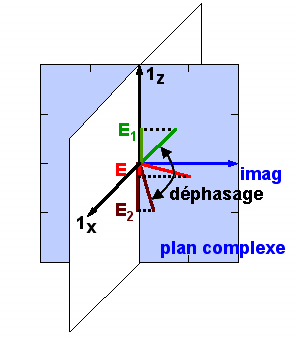
\includegraphics[scale=0.8]{M1}
\caption{Addition de 2 champs vectoriels complexes}
\label{M1}
\end{figure}

Utilisons à présent ce formalisme pour résoudre quantitativement un problème d'interférence. Un écran percé de $N$ fentes infiniment étroites séparées les unes des autres par la distance $d$, est illuminé par une onde plane\footnote{dans le plan $(x,y)$} arrivant sous incidence normale (voir fig. \ref{M2}).
\begin{figure}[htb]
\centering
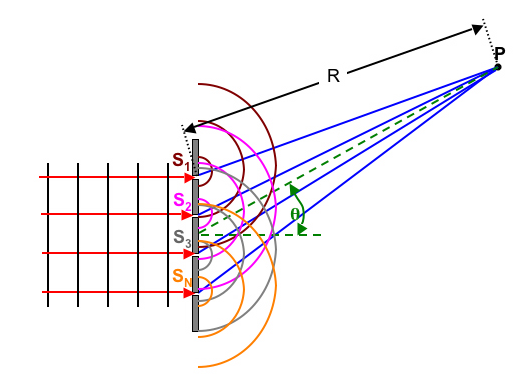
\includegraphics[scale=0.7]{M2}
\caption{Schéma des interférences issues d'une onde plane au travers d'un réseau de $N$ fentes}
\label{M2}
\end{figure}

\begin{marginfigure}[0cm]
	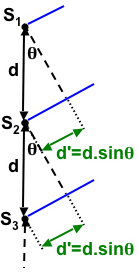
\includegraphics[scale=1]{M3}
	\caption{Retard de phase}
	\label{fm3}
\end{marginfigure}

Par l'approximation de Fraunhofer, le point $P$ où nous voulons calculer l'intensité se trouve très loin de l'écran. Nous pouvons alors considérer que les faisceaux bleus sont pratiquement parallèles. Chaque faisceau accuse un retard $d'$ par rapport au faisceau supérieur voisin (fig \ref{fm3}). La distance entre la source $S_p$ ($p=1,\ldots, N$) et le point $P$ est $R+(p-1)d'$.\\

Au point $P$, la superposition des faisceaux donne :
\begin{align*}
\overset\rightarrow{E}(P) & = \sum\limits_{p=1}^N \frac{A}{R+(p-1)d'}\exp\bigg(j\Big(k\big(R+(p-1)d'\big)-\omega t\Big)\bigg)\:\overset\rightarrow{\mbox{l}_z} \\
& = \exp\Big(j(kR-\omega t)\Big)\:\overset\rightarrow{\mbox{l}_z}\: \sum\limits_{p=1}^N \frac{A}{R+(p-1)d'}\exp(jk(p-1)d')
\end{align*}

Cette expression est simplement la somme des $N$ ondes sphériques émises par chaque fente, avec un repère placé de telle sorte que les champs soient parallèles à $\overset\rightarrow{\mbox{l}_z}$ en $P$. Le symbole $k$ est le nombre d'onde, $2\pi$ divisé par la longueur d'onde. Évidemment, le champ électrique correspond seulement à la partie réelle de cette expression, mais par souci de simplicité nous admettons que le symbole $\operatorname{Re}()$ est implicite dans ce qui suit.\\

Maintenant, la seule chose qu'il reste à faire est un développement mathématique de cette expression. Tout d'abord, l'approximation de Fraunhofer implique que $d' \ll R$. Dans ce cas, on peut considérer que 
$$\frac{A}{R+(p-1)d'} \simeq \frac{A}{R}.$$ 
Cette approximation n'est pas valide dans l'argument des exponentielles $jk(p-1)d' $, puisqu'une différence d'une demi-longueur d'onde est évidemment très importante quand il s'agit d'additionner des cosinus \footnote{ou des exponentielles complexes}. 
En se rappelant de la relation
$$\sum\limits_{p=0}^{N-1} x^p=\frac{1-x^N}{1-x}, $$
on écrit alors:
\begin{align*}
\overset\rightarrow{E}(P) & = \frac{A\exp\Big(j(kR-\omega t)\Big)}{R}\:\overset\rightarrow{\mbox{l}_z}\: \sum\limits_{p=1}^N \exp\Big(jk(p-1)d'\Big) \\
& =\frac{A\exp\Big(j(kR-\omega t)\Big)}{R}\:\overset\rightarrow{\mbox{l}_z}\: \sum\limits_{p=0}^{N-1} \exp(jkpd') \\
& = \frac{A\exp\Big(j(kR-\omega t)\Big)}{R}\:\overset\rightarrow{\mbox{l}_z}\: \sum\limits_{p=0}^{N-1} {\Big(\exp(jkd')\Big)}^{p} \\
& = \frac{A\exp\Big(j(kR-\omega t)\Big)}{R}\:\overset\rightarrow{\mbox{l}_z}\: 
\frac{1-{\Big(\exp(jkd')\Big)}^N}{1-\exp(jkd')}\\
& = \frac{A\exp\Big(j(kR-\omega t)\Big)}{R}\:\overset\rightarrow{\mbox{l}_z}\: 
\frac{1-\exp(jkNd')}{1-\exp(jkd')}
\end{align*}

Puisque $\exp(j\theta)+\exp(-j\theta)= 2\cos(\theta),$ l'intensité de l'onde résultante en $P$ est donnée par:
\begin{align*}
I(P) & =\frac{\epsilon c}{2}\overset\rightarrow{E_c}.\overset\rightarrow{E_c^*} \\
& = \frac{\epsilon c}{2}\frac{A^2}{R^2}\frac{\Big(1-\exp(jkNd')\Big)\Big(1-\exp(-jkNd')\Big)}{\Big(1-\exp(jkd')\Big)\Big(1-\exp(-jkd')\Big)}\\
& = \frac{\epsilon c}{2}\frac{A^2}{R^2}\frac{1-\exp(jkNd')-\exp(-jkNd')+1}{1-\exp(jkd')-\exp(-jkd')+1}\\
& = \frac{\epsilon c}{2}\frac{A^2}{R^2}\frac{2-2\cos(kNd')}{2-2\cos(kd')}\\
& = \frac{\epsilon c}{2}\frac{A^2}{R^2}\frac{1-\cos(kNd')}{1-\cos(kd')}\\
& = \frac{\epsilon c}{2}\frac{A^2}{R^2}\frac{2\sin^2(\frac{kNd'}{2})}{2\sin^2(\frac{kd'}{2})}\\
& = \frac{\epsilon c}{2}\frac{A^2}{R^2}\frac{\sin^2(\frac{N\pi d\sin\theta}{\lambda})}{\sin^2(\frac{\pi d\sin\theta}{\lambda})}
\end{align*}

Cette expression montre que l'intensité diminue en fonction du carré de la distance entre les fentes et le point $P$. De plus, le numérateur passe régulièrement par zéro, chaque fois que $N\pi d\sin\theta/\lambda$ vaut un multiple de $\pi$, c'est-à dire quand 
$$  d\sin\theta=\frac{m}{N}\lambda$$
où $m$ est un nombre entier. Ces conditions correspondent en général à des situations dans lesquelles les ondes interfèrent globalement de manière destructive, sauf pour une série de cas particuliers. Ces cas particuliers correspondent aux conditions $$d\sin \theta=n\lambda$$
où $n$ est un autre nombre entier. Si cette condition supplémentaire est vérifiée, le dénominateur de l'expression précédente tend vers zéro également, et la limite du quotient vaut\footnote{pour $\theta$ tendant vers $0$, le résultat étant similaire pour les autres pics}
\begin{align*}
\lim\limits_{\theta \rightarrow 0}\frac{\sin^2(\frac{N\pi d\sin\theta}{\lambda})}{\sin^2(\frac{\pi d\sin\theta}{\lambda})} & \overset{\frac{0}{0}}{=}\lim\limits_{\theta \rightarrow 0}\frac{2\sin(\frac{N\pi d\sin\theta}{\lambda})\frac{N\pi d\cos\theta}{\lambda}}{2\sin(\frac{\pi d\sin\theta}{\lambda})\frac{\pi d\cos\theta}{\lambda}} \\
& =\lim\limits_{\theta \rightarrow 0}\frac{\sin(\frac{N\pi d\sin\theta}{\lambda})N}{\sin(\frac{\pi d\sin\theta}{\lambda})}\\
& \overset{\frac{0}{0}}{=}\lim\limits_{\theta \rightarrow 0}\frac{\cos(\frac{N\pi d\sin\theta}{\lambda})\frac{N^2\pi d\cos\theta}{\lambda}}{\cos(\frac{\pi d\sin\theta}{\lambda})\frac{\pi d\cos\theta}{\lambda}}\\
& = N^2.
\end{align*}

L'intensité est alors $(\epsilon c/2)(NA/R)^2$, et les ondes interfèrent toutes ensemble de manière constructive en $P$. Ces directions correspondent à des maxima et la largeur du lobe\sidenote[][-1cm]{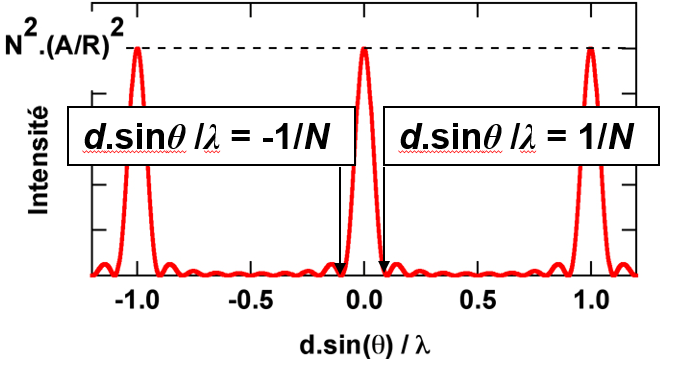
\includegraphics[scale=0.3]{M15}} associé est déterminé par
$$d\sin\theta/\lambda=2/N,$$
un nombre élevé de fentes ($N\uparrow\uparrow$) engendre donc des raies très étroites ($\theta\downarrow\downarrow$). Un nombre élevé des fentes implique aussi des maximas très élevés. Il est utile de se souvenir que, puisque ces maximas correspondent toujours à une situation où les $N$ sources sont en phase, ce maximum correspond toujours à une amplitude $N$ fois plus grande, et donc une intensité $N^2$ fois plus grande que ce qui serait reçu avec une seule source.

La figure \ref{M4} représente graphiquement l'intensité pour $10$ fentes.
\begin{figure}[htb]
\centering
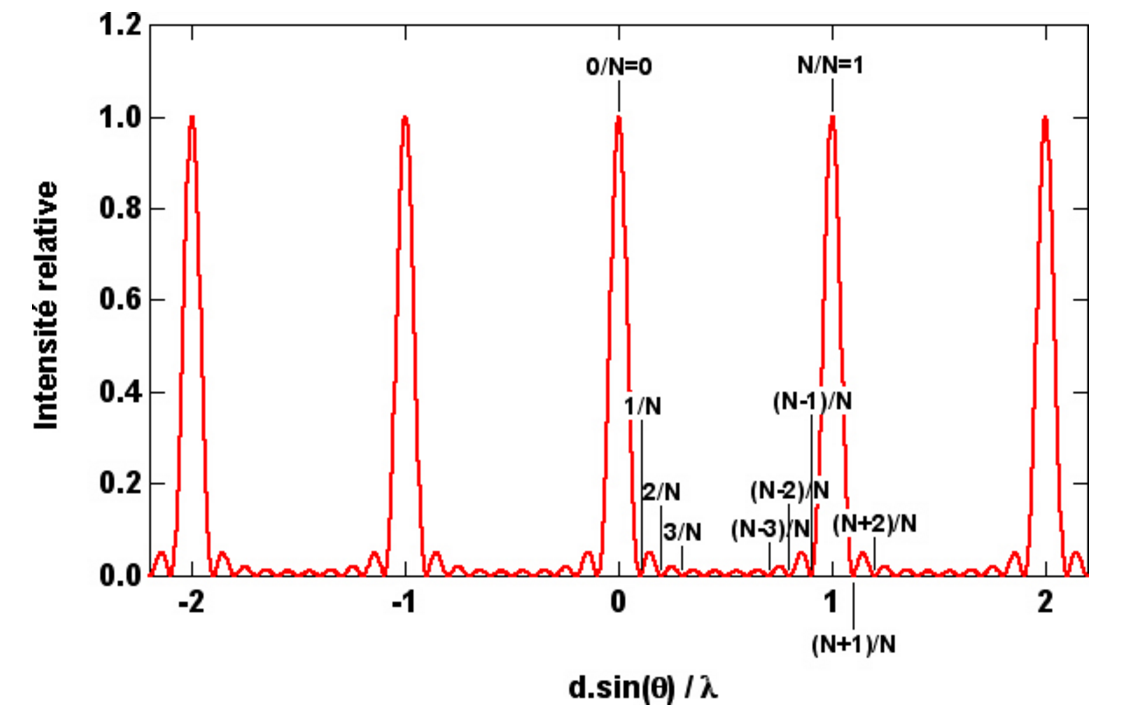
\includegraphics[scale=0.33]{M4}
\caption{Graphique de l'intensité selon l'angle de direction par rapport à la normale d'une onde passant à travers un réseau de 10 fentes }
\label{M4}
\end{figure}

Il y a un grand nombre de possibilités de combiner les différents faisceaux pour arriver à une intensité nulle, tandis que les cas correspondant à l'interférence constructive de tous les faisceaux sont plus rares. Nous avons considéré des fentes infiniment étroites; en général, il faut prendre en compte une largeur finie de fente, et un facteur supplémentaire s'introduit dans les expressions \footnote{voir chapitre lié à la diffraction}.

